\documentclass[../../main.tex]{subfiles}

\begin{document}

\chapter{Projective Geometry}



\section{Desargues' Theorem}

Desargues' Theorem is a renowned theorem that relates the axis and
the centers of perspective of two triangles. Therefore, before we dive
into Desargues' Theorem, we need to have a gut feeling on Projective
Geometry.

First, consider the two, not necessarily similar, triangles
and a point $P$.

\begin{figure}[H]
\centering
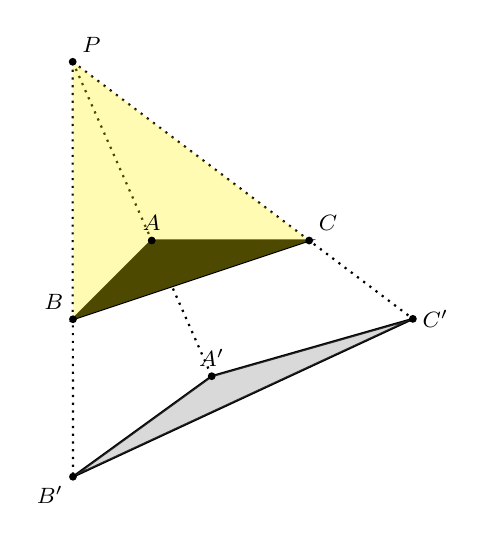
\begin{tikzpicture}[scale=0.2]
    \coordinate (A) at (5, 15);
    \coordinate (B) at (0, 10);
    \coordinate (C) at (15, 15);
    \coordinate (A') at (8.81, 6.384);
    \coordinate (B') at (0, 0);
    \coordinate (C') at (21.585, 10.024);
    \coordinate (P) at (-0.018, 26.349);
    \coordinate (G) at (-36.326, -26.326);
    \coordinate (I) at (39.052, 15);
    \coordinate (H) at (76.3, 35.433);

    \draw[thick] (A) -- (B) -- (C) -- (A);
    \draw[thick] (A') -- (B') -- (C') -- (A');

    \draw[thick, dotted] (P) -- (A');
    \draw[thick, dotted] (P) -- (B');
    \draw[thick, dotted] (P) -- (C');

    \fill[black] (A) -- (B) -- (C);
    \fill[yellow, opacity=0.3] (P) -- (B) -- (C);
    \fill[gray, opacity=0.3] (A') -- (B') -- (C');

    \foreach \n in {A, B, C, A', B', C', P}
    \node at (\n)[circle,fill,inner sep=1pt]{};

    \node[above] at (A) {\footnotesize $A$};
    \node[above left] at (B) {\footnotesize $B$};
    \node[above right] at (C) {\footnotesize $C$};
    \node[above] at (A') {\footnotesize $A'$};
    \node[below left] at (B') {\footnotesize $B'$};
    \node[right] at (C') {\footnotesize $C'$};
    \node[above right] at (P) {\footnotesize $P$};
\end{tikzpicture}
\caption{}
\label{fig:Desargues Theorem Figure 1}
\end{figure}

From the diagram above, we can think of it as having a light source
$P$ that shines $\triangle{ABC}$. There, we get our outcome
$\triangle{A'B'C'}$. Henceforth, we say that $A', B', C'$ are
corresponding points of $A, B, C$ respectively. Similarly, we could
state that $\overline{A'B'}, \overline{B'C'}, \overline{C'A'}$ are
corresponding sides of $\overline{AB}, \overline{BC}, \overline{CA}$
respectively.

\begin{theorem}
{Desargues' Theorem}
{Desargues' Theorem}
Two triangles are axially perspective if and only if they are
centrally perspective. Two triangles are considered axially
perspective if there exists the axis of perspectivity and they are
centrally perspective if there exists the center of perspectivity.
\end{theorem}

For simpler explanation, consider the diagram below, which is simply
the extension of Figure \ref{fig:Desargues Theorem Figure 1}.

\begin{figure}[H]
\centering
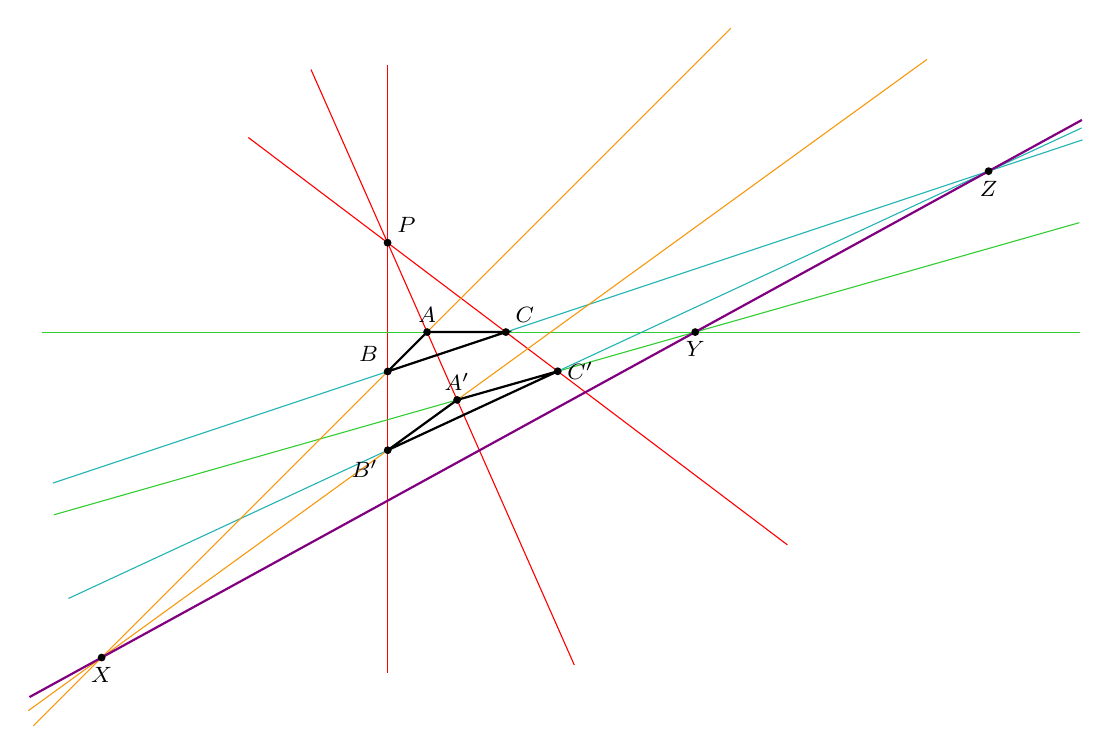
\begin{tikzpicture}[scale=0.1]
    \coordinate (A) at (5, 15);
    \coordinate (B) at (0, 10);
    \coordinate (C) at (15, 15);
    \coordinate (A') at (8.81, 6.384);
    \coordinate (B') at (0, 0);
    \coordinate (C') at (21.585, 10.024);
    \coordinate (P) at (-0.018, 26.349);
    \coordinate (X) at (-36.326, -26.326);
    \coordinate (Y) at (39.052, 15);
    \coordinate (Z) at (76.3, 35.433);

    \draw[red] (-17.695, 39.707) -- (50.757, -12.021);
    \draw[red] (-9.742, 48.339) -- (23.695, -27.279);
    \draw[red] (0, 48.926) -- (0, -28.305);

    \draw[LimeGreen] (-43.959, 15) -- (87.893, 15);
    \draw[LimeGreen] (-42.399, -8.204) -- (87.824, 28.894);
    \draw[TealBlue] (-42.509, -4.17) -- (88.226, 39.409);
    \draw[TealBlue] (-40.544, -18.828) -- (88.117, 40.921);
    \draw[YellowOrange]
        (-45.653, -33.086) -- (68.479, 49.628);
    \draw[YellowOrange]
        (-45, -35) -- (43.588, 53.588);

    \draw[thick, violet]
        (-45.498, -31.355) -- (88.156, 41.935);

    \draw[thick] (A) -- (B) -- (C) -- (A);
    \draw[thick] (A') -- (B') -- (C') -- (A');

    \foreach \n in {A, B, C, A', B', C', X, Y, Z, P}
    \node at (\n)[circle,fill,inner sep=1pt]{};

    \node[above] at (A) {\footnotesize $A$};
    \node[above left] at (B) {\footnotesize $B$};
    \node[above right] at (C) {\footnotesize $C$};
    \node[above] at (A') {\footnotesize $A'$};
    \node[below left] at (B') {\footnotesize $B'$};
    \node[right] at (C') {\footnotesize $C'$};
    \node[above right] at (P) {\footnotesize $P$};
    \node[below] at (X) {\footnotesize $X$};
    \node[below] at (Y) {\footnotesize $Y$};
    \node[below] at (Z) {\footnotesize $Z$};
\end{tikzpicture}
\caption{}
\label{fig:Figure 2}
\end{figure}

Point $P$, where $AA', BB', CC'$ concur, is the center of
perspectivity. Line $XZ$, where $X, Y, Z$ are collinear, is the axis
of perspectivity in the diagram above. If the pairs of corresponding
lines are all parallel, it is said that the lines meet at a point of
infinity. However, we normally don't discuss about that case.

The theorem is stating that if there exists a point $P$ such that
$P = AA' \cap BB' \cap CC'$, then the points $X = AB \cap A'B'$,
$Y = BC \cap B'C'$, and $Z = CA \cap C'A'$ are collinear.

Below is a quick example problem.

\begin{problem}{}{}
$D$ is a point on $\overline{BC}$ in $\triangle{ABC}$. Let $I_1$,
$I_2$ be the incenter of $\triangle{ABD}$ and $\triangle{ACD}$
respectively. Moreover, let $I_3$ and $I_4$ be ex-centers in
respect to $\angle{BAD}$ and $\angle{CAD}$ respectively. Show that
$\overline{I_1 I_2}$, $\overline{I_3 I_4}$, and $\overline{BC}$
intersect at one point.
\end{problem}
(\href{https://www.youtube.com/watch?v=adwiSgEAIG0}{Video Solution})
\begin{proof}
First, because $I_1$ and $I_2$ are the angle bisectors of
$\angle{ABD}$ and $\angle{ACD}$ respectively, $I = BI_1 \cap CI_2$
is the incenter of $\triangle{ABC}$. Similarly, we know that $I' =
BI_3 \cap CI_4$ is the ex-center of $\triangle{ABC}$ in respect that
$\angle{BAC}$. Therefore $A$, $I$, and $I'$ are collinear.

With similar idea, we could prove that $A, I_1, I_3$ are collinear
as well as $A, I_2, I_4$. In other words, $I_1I_3$ and $I_2I_4$
intersect at point $A$. Therefore, $BI_1 \cap CI_2$, $I_1I_3 \cap
I_2I_4$, and $I_3B \cap I_4C$ are collinear in $\triangle{I_1BI_3}$
and $\triangle{I_2CI_4}$. By Desargues' theorem, $\overline{I_1 I_2}$,
$\overline{I_3 I_4}$, and $\overline{BC}$ concurs.
\end{proof}

\subsection{Proof of Desargues' Theorem}

Let's try to prove the theorem. The proof involves the use of
Menelaus' theorem three times \cite{MATH01-1}.

\begin{proof}
First and foremost, recall that Menelaus' Theorem states the
following.

\begin{theorem}
{Menelaus' Theorem}
{Menelaus' Theorem}
Assume for $\triangle{ABC}$, $X, Y, Z$ are defined as $X \in
\overline{AB}$, $Y \in \overline{BC}$, and $Z \in \overline{CA}$.
Then, the following equation of cross-ratio holds.
\[
\frac{XA}{XB} \cdot \frac{YB}{YC} \cdot \frac{ZC}{ZA} = -1
\]
\end{theorem}

Because Desargues' Theorem must satisfy the if and only if condition,
let's first prove that two triangles are axially perspective if they
are centrally perspective.

Assuming that $\triangle{ABC}$ and $\triangle{A'B'C'}$ are perspective
from point $P$, Menelaus' Theorem could be used.

\begin{minipage}{0.48\textwidth}
\begin{center}
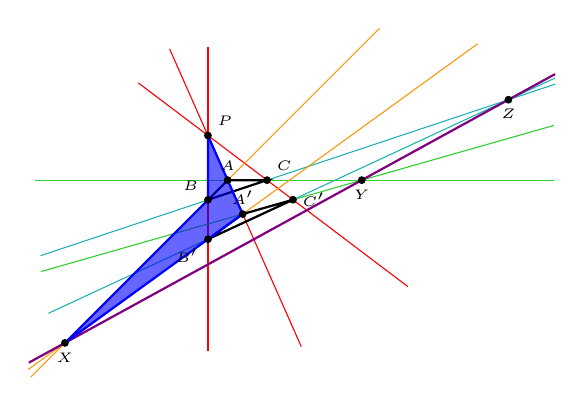
\begin{tikzpicture}[scale=0.05]
    \coordinate (A) at (5, 15);
    \coordinate (B) at (0, 10);
    \coordinate (C) at (15, 15);
    \coordinate (A') at (8.81, 6.384);
    \coordinate (B') at (0, 0);
    \coordinate (C') at (21.585, 10.024);
    \coordinate (P) at (-0.018, 26.349);
    \coordinate (X) at (-36.326, -26.326);
    \coordinate (Y) at (39.052, 15);
    \coordinate (Z) at (76.3, 35.433);

    \draw[red] (-17.695, 39.707) -- (50.757, -12.021);
    \draw[red] (-9.742, 48.339) -- (23.695, -27.279);
    \draw[red] (0, 48.926) -- (0, -28.305);

    \draw[LimeGreen] (-43.959, 15) -- (87.893, 15);
    \draw[LimeGreen] (-42.399, -8.204) -- (87.824, 28.894);
    \draw[TealBlue] (-42.509, -4.17) -- (88.226, 39.409);
    \draw[TealBlue] (-40.544, -18.828) -- (88.117, 40.921);
    \draw[YellowOrange]
        (-45.653, -33.086) -- (68.479, 49.628);
    \draw[YellowOrange]
        (-45, -35) -- (43.588, 53.588);

    \draw[thick, violet]
        (-45.498, -31.355) -- (88.156, 41.935);

    \draw[thick] (A) -- (B) -- (C) -- (A);
    \draw[thick] (A') -- (B') -- (C') -- (A');
    \draw[thick, blue]
        (P) -- (A) -- (A') -- (X) -- (B) -- (P);

    \fill[blue, opacity=0.6]
        (P) -- (A) -- (A') -- (X) -- (B);

    \foreach \n in {A, B, C, A', B', C', X, Y, Z, P}
        \node at (\n)[circle,fill,inner sep=1pt]{};

    \node[above] at (A) {\tiny $A$};
    \node[above left] at (B) {\tiny $B$};
    \node[above right] at (C) {\tiny $C$};
    \node[above] at (A') {\tiny $A'$};
    \node[below left] at (B') {\tiny $B'$};
    \node[right] at (C') {\tiny $C'$};
    \node[above right] at (P) {\tiny $P$};
    \node[below] at (X) {\tiny $X$};
    \node[below] at (Y) {\tiny $Y$};
    \node[below] at (Z) {\tiny $Z$};
\end{tikzpicture}
\end{center}
\end{minipage}
\hfill
\begin{minipage}{0.48\textwidth}
Consider $\triangle{PA'B'}$ with transverse line $XB$. Using Menelaus'
Theorem, the following equation could be derived.
\[
\frac{XA'}{XB'} \cdot \frac{BB'}{BP} \cdot \frac{AP}{AA'}
= 1
\]
\end{minipage}

\begin{minipage}{0.48\textwidth}
\begin{center}
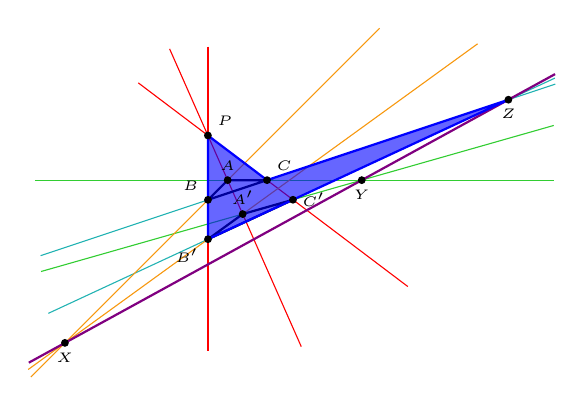
\begin{tikzpicture}[scale=0.05]
    \coordinate (A) at (5, 15);
    \coordinate (B) at (0, 10);
    \coordinate (C) at (15, 15);
    \coordinate (A') at (8.81, 6.384);
    \coordinate (B') at (0, 0);
    \coordinate (C') at (21.585, 10.024);
    \coordinate (P) at (-0.018, 26.349);
    \coordinate (X) at (-36.326, -26.326);
    \coordinate (Y) at (39.052, 15);
    \coordinate (Z) at (76.3, 35.433);

    \draw[red] (-17.695, 39.707) -- (50.757, -12.021);
    \draw[red] (-9.742, 48.339) -- (23.695, -27.279);
    \draw[red] (0, 48.926) -- (0, -28.305);

    \draw[LimeGreen] (-43.959, 15) -- (87.893, 15);
    \draw[LimeGreen] (-42.399, -8.204) -- (87.824, 28.894);
    \draw[TealBlue] (-42.509, -4.17) -- (88.226, 39.409);
    \draw[TealBlue] (-40.544, -18.828) -- (88.117, 40.921);
    \draw[YellowOrange]
        (-45.653, -33.086) -- (68.479, 49.628);
    \draw[YellowOrange]
        (-45, -35) -- (43.588, 53.588);

    \draw[thick, violet]
        (-45.498, -31.355) -- (88.156, 41.935);

    \draw[thick] (A) -- (B) -- (C) -- (A);
    \draw[thick] (A') -- (B') -- (C') -- (A');
    \draw[thick, blue]
        (P) -- (B') -- (C') -- (Z) -- (C) -- (P);

    \fill[blue, opacity=0.6]
        (P) -- (B') -- (C') -- (Z) -- (C);

    \foreach \n in {A, B, C, A', B', C', X, Y, Z, P}
        \node at (\n)[circle,fill,inner sep=1pt]{};

    \node[above] at (A) {\tiny $A$};
    \node[above left] at (B) {\tiny $B$};
    \node[above right] at (C) {\tiny $C$};
    \node[above] at (A') {\tiny $A'$};
    \node[below left] at (B') {\tiny $B'$};
    \node[right] at (C') {\tiny $C'$};
    \node[above right] at (P) {\tiny $P$};
    \node[below] at (X) {\tiny $X$};
    \node[below] at (Y) {\tiny $Y$};
    \node[below] at (Z) {\tiny $Z$};
\end{tikzpicture}
\end{center}
\end{minipage}
\hfill
\begin{minipage}{0.48\textwidth}
Similarly, consider $\triangle{PB'C'}$ and transverse line $ZC$.
\[
\frac{ZB'}{ZC'} \cdot \frac{CC'}{CP} \cdot \frac{BP}{BB'}
= 1
\]
\end{minipage}

\begin{minipage}{0.48\textwidth}
\begin{center}
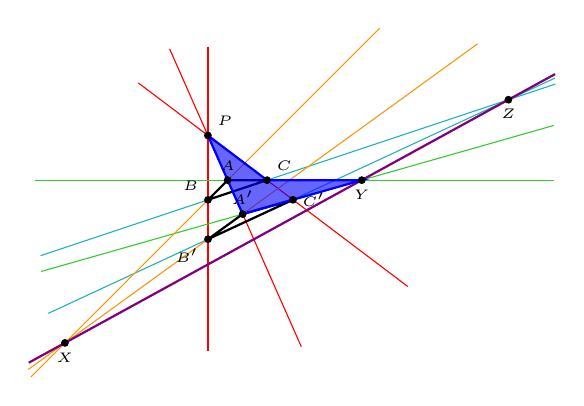
\begin{tikzpicture}[scale=0.05]
    \coordinate (A) at (5, 15);
    \coordinate (B) at (0, 10);
    \coordinate (C) at (15, 15);
    \coordinate (A') at (8.81, 6.384);
    \coordinate (B') at (0, 0);
    \coordinate (C') at (21.585, 10.024);
    \coordinate (P) at (-0.018, 26.349);
    \coordinate (X) at (-36.326, -26.326);
    \coordinate (Y) at (39.052, 15);
    \coordinate (Z) at (76.3, 35.433);

    \draw[red] (-17.695, 39.707) -- (50.757, -12.021);
    \draw[red] (-9.742, 48.339) -- (23.695, -27.279);
    \draw[red] (0, 48.926) -- (0, -28.305);

    \draw[LimeGreen] (-43.959, 15) -- (87.893, 15);
    \draw[LimeGreen] (-42.399, -8.204) -- (87.824, 28.894);
    \draw[TealBlue] (-42.509, -4.17) -- (88.226, 39.409);
    \draw[TealBlue] (-40.544, -18.828) -- (88.117, 40.921);
    \draw[YellowOrange]
        (-45.653, -33.086) -- (68.479, 49.628);
    \draw[YellowOrange]
        (-45, -35) -- (43.588, 53.588);

    \draw[thick, violet]
        (-45.498, -31.355) -- (88.156, 41.935);

    \draw[thick] (A) -- (B) -- (C) -- (A);
    \draw[thick] (A') -- (B') -- (C') -- (A');
    \draw[thick, blue]
        (P) -- (A') -- (C') -- (Y) -- (C) -- (P);

    \fill[blue, opacity=0.6]
        (P) -- (A') -- (C') -- (Y) -- (C);

    \foreach \n in {A, B, C, A', B', C', X, Y, Z, P}
        \node at (\n)[circle,fill,inner sep=1pt]{};

    \node[above] at (A) {\tiny $A$};
    \node[above left] at (B) {\tiny $B$};
    \node[above right] at (C) {\tiny $C$};
    \node[above] at (A') {\tiny $A'$};
    \node[below left] at (B') {\tiny $B'$};
    \node[right] at (C') {\tiny $C'$};
    \node[above right] at (P) {\tiny $P$};
    \node[below] at (X) {\tiny $X$};
    \node[below] at (Y) {\tiny $Y$};
    \node[below] at (Z) {\tiny $Z$};
\end{tikzpicture}
\end{center}
\end{minipage}
\hfill
\begin{minipage}{0.48\textwidth}
With $\triangle{PC'A'}$ and line $YC$,
\begin{align*}
    \frac{YA'}{YC'} \cdot \frac{CC'}{CP}
    \cdot \frac{AP}{AA'}
    &= 1 \\
    \frac{YC'}{YA'} \cdot \frac{CP}{CC'}
    \cdot \frac{AA'}{AP}
    &= 1
\end{align*}
\end{minipage}

Multiplying the equations,
\begin{align*}
    \left( \frac{XA'}{XB'} \cdot \frac{BB'}{BP}
        \cdot \frac{AP}{AA'} \right) \cdot
    \left( \frac{ZB'}{ZC'} \cdot \frac{CC'}{CP}
        \cdot \frac{BP}{BB'} \right) \cdot
    \left( \frac{YC'}{YA'} \cdot \frac{CP}{CC'}
        \cdot \frac{AA'}{AP} \right)
    &= 1 \\
    \frac{XA'}{XB'} \cdot \frac{ZB'}{ZC'} \cdot
    \frac{YC'}{YA'}
    &= 1
\end{align*}
is obtained. Continuing, consider the following diagrams.

\begin{center}
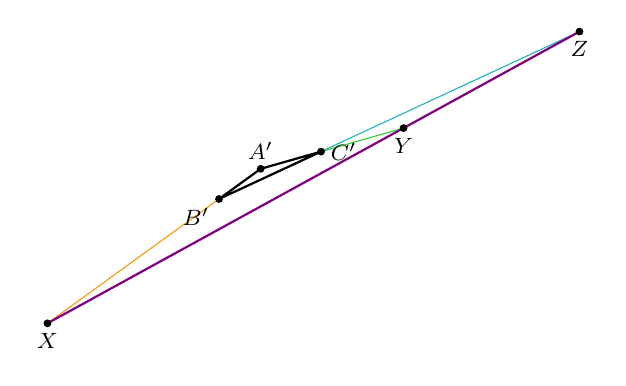
\begin{tikzpicture}[scale=0.06]
    \coordinate (A') at (8.81, 6.384);
    \coordinate (B') at (0, 0);
    \coordinate (C') at (21.585, 10.024);
    \coordinate (X) at (-36.326, -26.326);
    \coordinate (Y) at (39.052, 15);
    \coordinate (Z) at (76.3, 35.433);

    \draw[LimeGreen] (A') -- (Y);
    \draw[TealBlue] (B') -- (Z);
    \draw[YellowOrange] (X) -- (A');

    \draw[thick, violet] (X) -- (Z);

    \draw[thick] (A') -- (B') -- (C') -- (A');

    \foreach \n in {A', B', C', X, Y, Z}
        \node at (\n)[circle,fill,inner sep=1pt]{};

    \node[above] at (A') {\footnotesize $A'$};
    \node[below left] at (B') {\footnotesize $B'$};
    \node[right] at (C') {\footnotesize $C'$};
    \node[below] at (X) {\footnotesize $X$};
    \node[below] at (Y) {\footnotesize $Y$};
    \node[below] at (Z) {\footnotesize $Z$};
\end{tikzpicture}
\end{center}

By converse of Menelaus' Theorem, it is evident that $X$, $Y$, and
$Z$ are collinear.

Now that the first statement for if and only if condition is proven,
the converse must also be proven. Consider the diagram below where the
same construction method is used. Note that if $AA'$, $BB'$, and $CC'$
concur is yet to be known.

\begin{center}
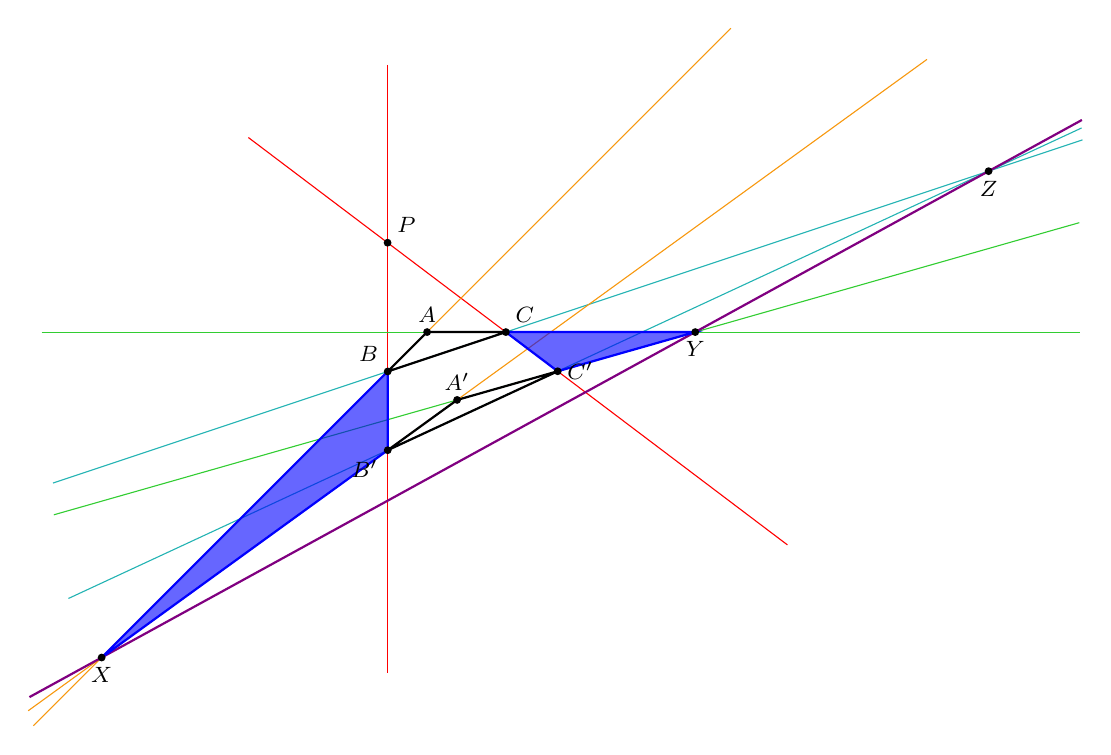
\begin{tikzpicture}[scale=0.1]
    \coordinate (A) at (5, 15);
    \coordinate (B) at (0, 10);
    \coordinate (C) at (15, 15);
    \coordinate (A') at (8.81, 6.384);
    \coordinate (B') at (0, 0);
    \coordinate (C') at (21.585, 10.024);
    \coordinate (P) at (-0.018, 26.349);
    \coordinate (X) at (-36.326, -26.326);
    \coordinate (Y) at (39.052, 15);
    \coordinate (Z) at (76.3, 35.433);

    \draw[red] (-17.695, 39.707) -- (50.757, -12.021);
    \draw[red] (0, 48.926) -- (0, -28.305);

    \draw[LimeGreen] (-43.959, 15) -- (87.893, 15);
    \draw[LimeGreen] (-42.399, -8.204) -- (87.824, 28.894);
    \draw[TealBlue] (-42.509, -4.17) -- (88.226, 39.409);
    \draw[TealBlue] (-40.544, -18.828) -- (88.117, 40.921);
    \draw[YellowOrange]
        (-45.653, -33.086) -- (68.479, 49.628);
    \draw[YellowOrange]
        (-45, -35) -- (43.588, 53.588);

    \draw[thick, violet]
        (-45.498, -31.355) -- (88.156, 41.935);

    \draw[thick] (A) -- (B) -- (C) -- (A);
    \draw[thick] (A') -- (B') -- (C') -- (A');
    \draw[thick, blue] (B) -- (B') -- (X) -- (B);
    \draw[thick, blue] (C) -- (C') -- (Y) -- (C);

    \fill[blue, opacity=0.6] (B) -- (B') -- (X);
    \fill[blue, opacity=0.6] (C) -- (C') -- (Y);

    \foreach \n in {A, B, C, A', B', C', X, Y, Z, P}
        \node at (\n)[circle,fill,inner sep=1pt]{};

    \node[above] at (A) {\footnotesize $A$};
    \node[above left] at (B) {\footnotesize $B$};
    \node[above right] at (C) {\footnotesize $C$};
    \node[above] at (A') {\footnotesize $A'$};
    \node[below left] at (B') {\footnotesize $B'$};
    \node[right] at (C') {\footnotesize $C'$};
    \node[above right] at (P) {\footnotesize $P$};
    \node[below] at (X) {\footnotesize $X$};
    \node[below] at (Y) {\footnotesize $Y$};
    \node[below] at (Z) {\footnotesize $Z$};
\end{tikzpicture}
\end{center}

Notice that $\triangle{XBB'}$ and $\triangle{YCC'}$ are in
perspective from point $Z$. Moreover, the first half of the proof
manifests that $P$, $A$, and $A'$ must be collinear. By construction,
$P$ is on line $BB'$ and $CC'$. Moreover, it is also on the line
$AA'$. Thus, $\triangle{ABC}$ and $\triangle{A'B'C'}$ are centrally
perspective if they are axially perspective.
\end{proof}

\end{document}

